\chapter{Usability Test}
Um die nicht funktionalen Anforderungen des Workflow Systems zu bewerten, wurde eine Benutzerumfrage durchgeführt. Dabei wurden insbesondere die Benutzerfreundlichkeit und diei intuitive  Bedienung der Anwendung betrachtet. Im Rahmen der Umfrage wurden den Benutzern vorgeschlagen das Worfklow System zu testen, indem sie einfache Workflows selbständig erstellen, speichern, ausführen und bearbeiten. Insgesamt haben 17 Personen an der Umfrage teilgenommen. In diesem Kapitel werden die Ergebnisse der Benutzerumfrage vorgestellt.

\begin{figure}[H]
    \centering
    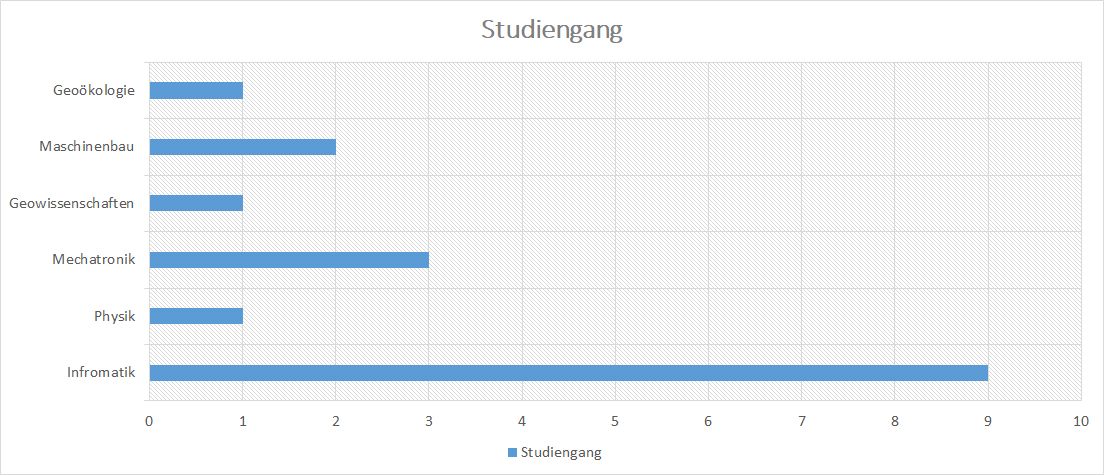
\includegraphics[width=15cm]{diagrams/TeilnehmerDiagramm.jpg}
    \caption{Teilnehmer}
    \label{teilnehmer}
\end{figure}

\section{Inhalt der Umfrage}
Die Aufgabe war einige arithmetische Gleichungen mit Hilfe des Workflow Systems zu lösen. Dazu haben die Benutzer eine kurze Einleitung gelesen, in der die Hauptkonzepte des Systems erklärt wurden. Danach sollte der Befragte zunächst den Server hinfügen um die arithmetischen Operationen ausführen zu können.\newline
Danach sollte der Benutzer die folgenden Gleichungen lösen:

\begin{enumerate}
    \item \(500  \times (5 + 5)\) Antwort: 5000
    \item \((3 + 8)^2 - 4 \times 10\) Antwort: 81 \newline
    Nächste Gleichung muss jetzt nicht von Anfang an als Workflow gemacht werden, sondern man muss den existierenden Workflow entsprechend bearbeiten.
    \item \((3 + 8)^2 + 4 \times 10\) Antwort: 161
    \item \(\frac{(10 + 2) \times 3}{9 - 2 - 1}\) Antwort: 6
\end{enumerate}
Nachdem die Gleichungen richtig gelöst sind, soll der Befragte einen Fragebogen ausfüllen, um das System zu bewerten.



\newpage

\section{Ergebnisse}
Im folgenden sind die Ergebnisse der Umfrage aufgelistet. \newline
Die Befragten sollten bewerten, ob die folgenden Aussagen voll (Note 10) oder überhaupt nicht (Note 1) zutreffen. \newline
Insgesamt wurde die Bedienbarkeit von allen Testpersonen als normal bis einfach eingestuft.
\begin{figure}[H]
    \centering
    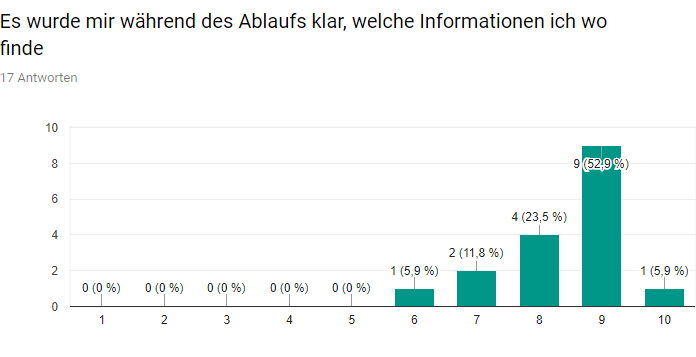
\includegraphics[width=15cm]{diagrams/ErgebnisStat1.jpg}
    \label{Ergebnis1}
\end{figure}

\begin{figure}[H]
    \centering
    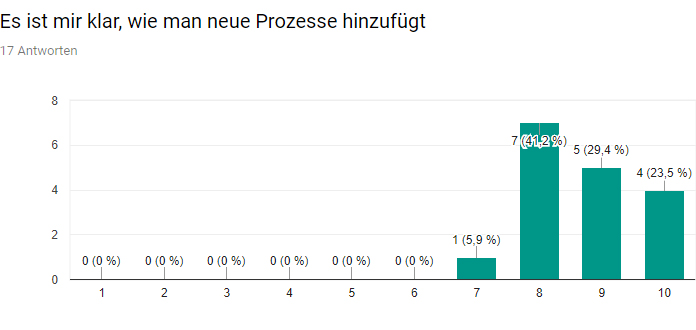
\includegraphics[width=15cm]{diagrams/ErgebnisStat2.jpg}
    \label{Ergebnis2}
\end{figure}

\begin{figure}[H]
    \centering
    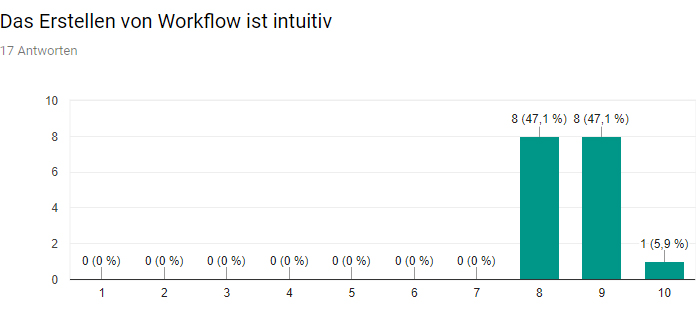
\includegraphics[width=15cm]{diagrams/ErgebnisStat3.jpg}
    \label{Ergebnis3}
\end{figure}

\begin{figure}[H]
    \centering
    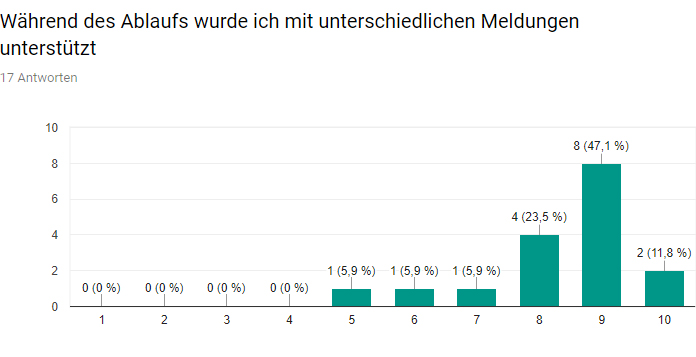
\includegraphics[width=15cm]{diagrams/ErgebnisStat4.jpg}
    \label{Ergebnis4}
\end{figure}

\begin{figure}[H]
    \centering
    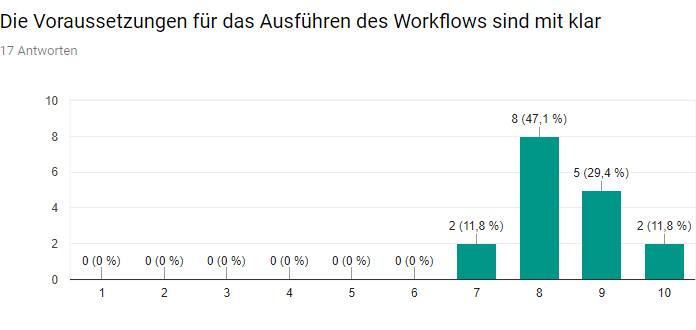
\includegraphics[width=15cm]{diagrams/ErgebnisStat5.jpg}
    \label{Ergebnis5}
\end{figure}

\begin{figure}[H]
    \centering
    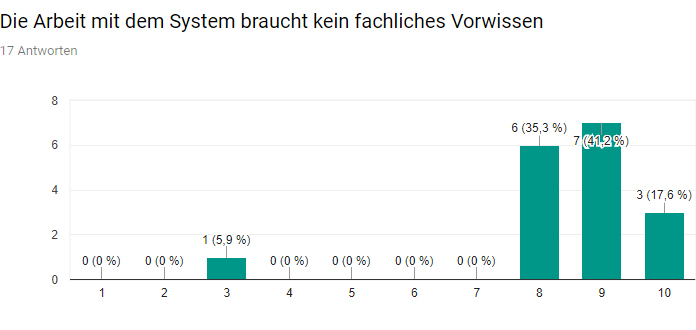
\includegraphics[width=15cm]{diagrams/ErgebnisStat6.jpg}
    \label{Ergebnis6}
\end{figure}

\begin{figure}[H]
    \centering
    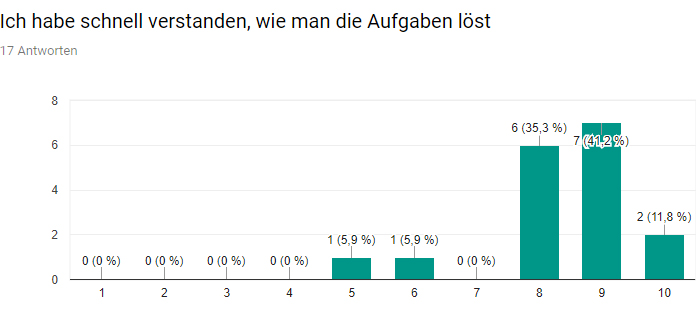
\includegraphics[width=15cm]{diagrams/ErgebnisStat7.jpg}
    \label{Ergebnis7}
\end{figure}

\begin{figure}[H]
    \centering
    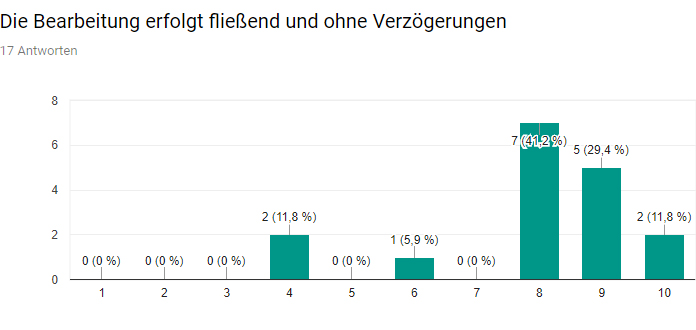
\includegraphics[width=15cm]{diagrams/ErgebnisStat8.jpg}
    \label{Ergebnis8}
\end{figure}

Folgende Kriterien wurden mit den Noten von 1 bis 6 bewertet, wobei 1 die beste und 6 die schlechteste Note ist.

\begin{figure}[H]
    \centering
    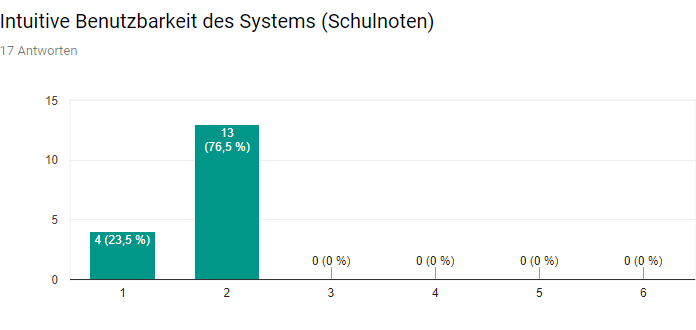
\includegraphics[width=15cm]{diagrams/ErgebnisStatSchul1.jpg}
    \label{ErgebnisSchul1}
\end{figure}

\begin{figure}[H]
    \centering
    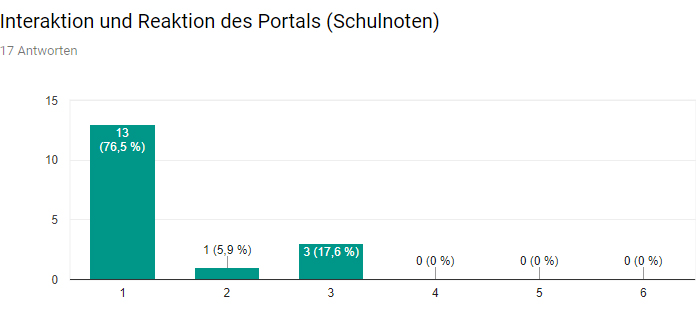
\includegraphics[width=15cm]{diagrams/ErgebnisStatSchul2.jpg}
    \label{ErgebnisSchul2}
\end{figure}

\begin{figure}[H]
    \centering
    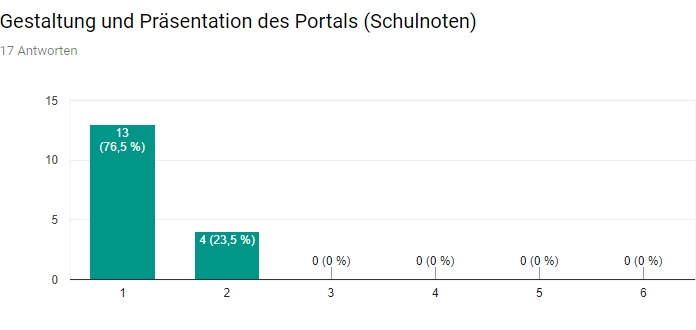
\includegraphics[width=15cm]{diagrams/ErgebnisStatSchul3.jpg}
    \label{ErgebnisSchul3}
\end{figure}

\begin{figure}[H]
    \centering
    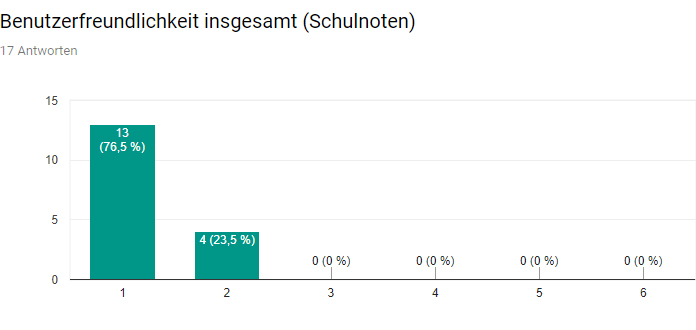
\includegraphics[width=15cm]{diagrams/ErgebnisStatSchul4.jpg}
    \label{ErgebnisSchul4}
\end{figure}